\documentclass[conference]{IEEEtran}
\IEEEoverridecommandlockouts
% The preceding line is only needed to identify funding in the first footnote. If that is unneeded, please comment it out.
\usepackage[T1]{fontenc}
\usepackage[utf8]{inputenc}
\usepackage[croatian]{babel}
\usepackage{cite}
\usepackage{amsmath,amssymb,amsfonts}
\usepackage{algorithmic}
\usepackage{graphicx}
\usepackage{textcomp}
\usepackage{xcolor}
\usepackage{booktabs}
\usepackage{pgfplots}
\pgfplotsset{compat=1.18}
\def\BibTeX{{\rm B\kern-.05em{\sc i\kern-.025em b}\kern-.08em
    T\kern-.1667em\lower.7ex\hbox{E}\kern-.125emX}}
\begin{document}

\title{Paralelizacija algoritama sortiranja: Optimizacija performansi kroz paralelno računarstvo}

\author{\IEEEauthorblockN{Harun Goralija}
\IEEEauthorblockA{\textit{Elektrotehnički fakultet} \\
\textit{Univerzitet u Sarajevu}\\
Sarajevo, Bosna i Hercegovina \\
hgoralija2@etf.unsa.ba}
\and
\IEEEauthorblockN{Belmin Durmo}
\IEEEauthorblockA{\textit{Elektrotehnički fakultet} \\
\textit{Univerzitet u Sarajevu}\\
Sarajevo, Bosna i Hercegovina \\
bdurmo1@etf.unsa.ba}
\and
\IEEEauthorblockN{Harun Mioc}
\IEEEauthorblockA{\textit{Elektrotehnički fakultet} \\
\textit{Univerzitet u Sarajevu}\\
Sarajevo, Bosna i Hercegovina \\
hmioc1@etf.unsa.ba}
\and
\IEEEauthorblockN{Amar Hodžić}
\IEEEauthorblockA{\textit{Elektrotehnički fakultet} \\
\textit{Univerzitet u Sarajevu}\\
Sarajevo, Bosna i Hercegovina \\
ahodzic13@etf.unsa.ba}
\and
\IEEEauthorblockN{Kenan Abadžić}
\IEEEauthorblockA{\textit{Elektrotehnički fakultet} \\
\textit{Univerzitet u Sarajevu}\\
Sarajevo, Bosna i Hercegovina \\
kabadzic1@etf.unsa.ba}
}

\maketitle

\begin{abstract}
Ovaj rad se bavi paralelizacijom algoritama sortiranja s ciljem optimizacije performansi kroz paralelno računarstvo. U eri velikih podataka, efikasno sortiranje velikih skupova podataka postaje ključno za aplikacije poput baza podataka i mašinskog učenja. Tradicionalni sekvencijalni algoritmi postaju usko grlo za velike skupove podataka.

Rad istražuje implementacije na višejezgrenim CPU-ima koristeći OpenMP i na GPU-ima koristeći CUDA. Implementirani su algoritmi: bitonic sort, merge sort, quick sort, radix sort i std::sort u sekvencijalnim i paralelnim varijantama.

Rezultati na 134 miliona elemenata pokazuju značajna ubrzanja, posebno za regularne algoritme poput radix sorta (21,6$\times$ na CPU, 386 Melem/s na GPU). Poređenje CPU i GPU implementacija ističe komplementarnu prirodu dvije platforme: GPU nadmašuje CPU za masovno paralelne workloade, dok CPU pruža konkurentne performanse za manje skupove podataka bez overhead-a memorijskih transfera.

Rad doprinosi razumijevanju primjene paralelnih tehnika na algoritme sortiranja i pruža uvide u optimizaciju performansi na modernom heterogenom hardveru.
\end{abstract}

\begin{IEEEkeywords}
paralelizacija, algoritmi sortiranja, paralelno računarstvo, CPU, GPU, OpenMP, CUDA
\end{IEEEkeywords}

\section{Introduction}

U eri velikih podataka, efikasno sortiranje postaje temelj mnogih računarskih aplikacija. Tradicionalni sekvencijalni algoritmi postižu složenost O(n log n), što je optimalno za sekvencijalne mašine, ali postaju usko grlo za velike skupove podataka.

Paralelizacija algoritama sortiranja predstavlja prirodno rješenje. Iskorištavanjem više procesorskih jezgara ili GPU-a, moguće je značajno ubrzati sortiranje. Ovaj rad fokusira se na paralelizaciju pet algoritama: bitonic sort, merge sort, quick sort, radix sort i std::sort, sa implementacijama na CPU (OpenMP) i GPU (CUDA). Ukupno je implementirano 25 varijanti (5 algoritama $\times$ 5 nivoa: naivni sekvencijalni, optimizovani sekvencijalni, paralelni CPU, naivni GPU i paralelni GPU) sa preko 6.700 linija koda.

Tema je relevantna jer paralelno računarstvo postaje neizbježno u aplikacijama poput analize velikih podataka i real-time procesiranja. Ključni izazov je mapiranje inherentno sekvencijalnih dijelova algoritama na masovno paralelne arhitekture, uz minimiziranje overhead-a sinhronizacije i memorijskih transfera.

Rad je organizovan na sljedeći način: Sekcija II daje pregled relevantne literature. Sekcija III opisuje implementaciju svih varijanti algoritama, uključujući sekvencijalne, optimizovane i paralelne verzije za CPU i GPU. Sekcija IV prezentira eksperimentalne rezultate sa detaljnim mjerenjima performansi. Sekcija V diskutuje rezultate i ograničenja, a Sekcija VI zaključuje rad.

\section{Literature Review}

Paralelno sortiranje je aktivno istraživano područje od 1960-ih, kada je Batcher uveo bitonic sort sa O(log² n) složenošću \cite{Batcher68}. Moderna istraživanja fokusiraju se na GPU implementacije, gdje algoritmi poput bitonic sorta postižu značajna ubrzanja zahvaljujući SIMD arhitekturi \cite{Schmid22}. Merge sort se dobro paralelizuje divide-and-conquer pristupom na višejezgrenim CPU-ima \cite{Mujic23}, dok quicksort izazove predstavlja zbog nebalansiranih particija, ali pokazuje dobre rezultate na GPU-ima za velike skupove podataka \cite{Catic23}. Radix sort, kao nekomparativni algoritam, postiže linearnu složenost i izuzetne performanse na GPU-ima \cite{Yazici20}.

Literatura naglašava prednosti heterogenog računarstva, gdje GPU implementacije nadmašuju CPU za masovno paralelne workload-e, ali CPU pruža bolju skalabilnost za manje podatke. NVIDIA Thrust biblioteka \cite{Schmid22} služi kao de facto standard za GPU sortiranje i pruža visokooptimizovane implementacije koje iskorištavaju specifične karakteristike svake GPU arhitekture. Ovaj rad doprinosi polju pružajući direktne implementacije i poređenja performansi pet algoritama na CPU (OpenMP) i GPU (CUDA) platformama, adresirajući praznine u sveobuhvatnim studijama paralelizacije.

\section{Implementation}

Projekat implementira pet algoritama sortiranja: bitonic sort, merge sort, quick sort, radix sort i std::sort. Svaki algoritam je realizovan u tri varijante: sekvencijalna (naivna), sekvencijalna optimizovana i paralelna CPU verzija koristeći OpenMP sa SIMD instrukcijama.

\subsection{Arhitektura projekta}

Implementacija je organizovana u modularnoj strukturi sa zajedničkim header fajlovima (\texttt{main\_template.hpp}, \texttt{timers.hpp}, \texttt{utils.hpp}) koji pružaju infrastrukturu za testiranje, mjerenje performansi i generisanje testnih podataka. Svaki algoritam ima svoj wrapper koji se integriše sa sistemom za benchmarking. Build sistem koristi CMake sa Ninja generatorom, a CPU kod se kompajlira sa GCC 13.2 uz \texttt{-O3 -march=native -mavx2} zastavice za maksimalnu optimizaciju.

\subsection{Sekvencijalne implementacije}

Sekvencijalne verzije služe kao baseline za poređenje performansi. Naivne implementacije koriste standardne rekurzivne pristupe: quick sort sa Lomuto particioniranjem, merge sort sa rekurzivnim spajanjem, bitonic sort sa rekurzivnim compare-and-swap mrežama, radix sort sa base-10 counting sortom po cifri, i standardni \texttt{std::sort}.

Optimizovane verzije uvode niz poboljšanja. Quick sort koristi Hoare particioniranje sa median-of-three pivotom i tail rekurzijom, sa prelaskom na insertion sort za nizove manje od 24 elementa. Merge sort prelazi na iterativni pristup sa ping-pong double-buffering tehnikom koja eliminira rekurziju i nepotrebno kopiranje. Radix sort koristi base-256 shemu (8-bitni prolazi) umjesto base-10, uz preskakanje prolaza kada su svi elementi jednaki na datom byte-u, što značajno ubrzava sortirane i blizu-sortirane nizove.

\subsection{Paralelne CPU implementacije}

Paralelne verzije koriste OpenMP za višejezgrenu paralelizaciju. Ključne optimizacije uključuju:

\textbf{Bitonic sort} kombinuje SIMD instrukcije (AVX2) za vektorizovane compare-and-swap operacije (\texttt{\_mm256\_min\_epi32}, \texttt{\_mm256\_max\_epi32}) sa OpenMP task paralelizmom za velike nizove. Procesira 8 parova elemenata po SIMD instrukciji i koristi insertion sort za sekvence manje od 128 elemenata.

\textbf{Merge sort} koristi Merge-Path algoritam koji binarnom pretragom dijeli posao ravnomjerno među nitima, čime se izbjegava problem nebalansiranog spajanja kod standardnog pristupa. Implementira 64-byte poravnanu alokaciju i AVX2-ubrzani \texttt{simd\_memcpy} za kopiranje podataka.

\textbf{Quick sort} implementira Dutch National Flag 3-way particioniranje za efikasno rukovanje duplikatima, sa AVX2 vektorskim prefetch-om i OpenMP task-ovima koji se dinamički kreiraju samo za particije veće od praga.

\textbf{Radix sort} koristi thread-local histograme za eliminaciju false sharing-a između niti. Svaka nit akumulira lokalni histogram za svoj dio niza, nakon čega se histogrami kombinuju u globalne prefiksne sume. Base-256 shema sa 4 prolaza (po 8 bitova) minimizira broj sinhronizacija, dok SIMD instrukcije ubrzavaju scatter fazu. Ova kombinacija čini radix sort najbrži paralelni algoritam na CPU-u.

\textbf{std::sort} paralelizuje postojeću C++ standardnu biblioteku koristeći \texttt{std::execution::par\_unseq} execution policy iz C++17 standarda, što kompajleru omogućava automatsku vektorizaciju i paralelizaciju bez eksplicitnog upravljanja nitima.

Implementacije koriste pragme kao \texttt{\#pragma omp parallel for} i \texttt{\#pragma omp task} za eksplicitnu paralelizaciju, sa pažljivim balansiranjem opterećenja i minimizacijom overhead-a sinhronizacije. Prag za kreiranje novih task-ova je ključan parametar: premali prag uzrokuje prevelik overhead kreiranja zadataka, dok preveliki prag rezultira nedovoljnom paralelizacijom.

\subsection{GPU implementacije}

GPU verzije koriste NVIDIA CUDA platformu za masivnu paralelizaciju na grafičkom procesoru RTX 3050 Ti Laptop GPU sa 20 streaming multiprocesora (SM) i compute capability 8.6. CUDA programski model organizuje niti u hijerarhiju: niti se grupišu u warp-ove (32 niti), blokove i grid, što omogućava fino upravljanje paralelizmom. Ključni optimizacijski ciljevi su koalescentan pristup memoriji, korištenje shared memorije i maksimalan occupancy.

\textbf{Bitonic sort} koristi dvofazni pristup. U prvoj fazi, shared memory kernel sortira blokove od 512 elemenata koristeći \texttt{\_\_shared\_\_} memoriju za brze compare-and-swap operacije unutar bloka. U drugoj fazi, za korake $k > 512$, koristi se global memory kernel sa grid-stride petljom koji sakriva latenciju pristupa globalnoj memoriji. Ulazni niz se dopunjava do sljedeće potencije broja 2 sa \texttt{INT\_MAX} vrijednostima.

\textbf{Merge sort} kombinuje bitonic sort kao bazni slučaj sa paralelnim merge-path algoritmom. Početno sortiranje blokova od 512 elemenata vrši se istim shared memory bitonic kernelom. Zatim se sortirani blokovi spajaju paralelnim merge kernelom koji koristi binarnu pretragu za određivanje pozicije svakog elementa u spajanju, čime se postiže ravnomjerna raspodjela posla. Implementirane su tri varijante: PerElement (jedan element po niti), Coarsened (više elemenata po niti za sakrivanje latencije) i BlockMerge. Double-buffering tehnikom se izbjegava nepotrebno kopiranje.

\textbf{Quick sort} koristi hibridni CPU-GPU pristup (Iterative V2). CPU vrši bootstrap fazu koristeći BFS particioniranje dok se ne kreira oko 65.536 zadataka, čime se izbjegava sekvencijalno usko grlo prvog nivoa rekurzije. GPU kernel zatim procesira zadatke koristeći warp-agregiranu task queue sa \texttt{\_\_ballot\_sync} i \texttt{\_\_shfl\_sync} primitivama za efikasnu distribuciju posla. Mali segmenti ($\leq 16$ elemenata) se sortiraju insertion sortom u registrima, a pivot se bira median-of-9 tehnikom za velike segmente.

\textbf{Radix sort} implementira LSB (Least Significant Bit) pristup procesiranjem po jednog bita u 32 prolaza. Count kernel koristi warp-level redukciju sa \texttt{\_\_shfl\_down\_sync} za brojanje nula po bloku. Scan kernel računa prefix sume za globalne offsete, a scatter kernel koristi \texttt{\_\_ballot\_sync} za efikasno raspoređivanje elemenata na izlazne pozicije. Implementacija se poredi sa NVIDIA Thrust bibliotekom kao baznom linijom.

Dodatno, implementirane su i naivne GPU verzije sa konfiguracijom \texttt{<<<1, 1>>>} (jedna nit) koje služe za demonstraciju overhead-a GPU kernel pokretanja i memorijskih transfera bez koristi od paralelizacije. Ove verzije su očekivano višestruko sporije od CPU naivnih implementacija, jer jedna GPU nit radi na nižoj frekvenciji (1,5 GHz) u poređenju sa CPU jezgrom (4,4 GHz), bez mogućnosti branch prediction-a i spekulativnog izvršavanja.

\section{Eksperimentalni rezultati}

\subsection{Testno okruženje}

Eksperimenti su izvršeni na sistemu sa AMD Ryzen 7 5800H procesorom (8 jezgara, 16 niti) i NVIDIA GeForce RTX 3050 Ti Laptop GPU (20 SM-ova, compute capability 8.6, 4 GB GDDR6). Operativni sistem je Windows, CPU kod je kompajliran sa GCC 13.2 uz optimizacije \texttt{-O3 -march=native -mavx2} i OpenMP 4.5, dok su GPU kerneli kompajlirani sa NVCC za \texttt{sm\_86} arhitekturu. Svi testovi koriste nasumično generirane nizove cijelih brojeva sa seed vrijednošću 12345 radi reproducibilnosti. CPU benchmarci su pokrenuti za veličine nizova od 16K do 128M elemenata, dok su GPU benchmarci izvršeni na 128M elemenata radi evaluacije performansi na velikim skupovima podataka.

\subsection{CPU rezultati}

Tabela~\ref{tab:cpu} prikazuje vremena izvršavanja za 134.217.728 (128M) elemenata na CPU-u. Za bitonic sort naivnu verziju prikazano je vrijeme na 8M elemenata jer je $O(n \log^2 n)$ složenost čini nepraktičnom za 128M.

\begin{table}[htbp]
\caption{CPU performanse sortiranja -- 128M random elementi (ms)}
\label{tab:cpu}
\centering
\small
\begin{tabular}{lrrrr}
\toprule
\textbf{Algoritam} & \textbf{Naivni} & \textbf{Opt.} & \textbf{Par. CPU} & \textbf{Ubrzanje} \\
\midrule
Bitonic sort & 2026\textsuperscript{*} & 33608 & 12511 & 1,0$\times$\textsuperscript{*} \\
Merge sort & 26266 & 11386 & 2768 & 9,5$\times$ \\
Quick sort & 12168 & 9647 & 1803 & 6,7$\times$ \\
Radix sort & 10885 & 1507 & 505 & 21,6$\times$ \\
std::sort & 8520 & 8342 & 1310 & 6,5$\times$ \\
\bottomrule
\multicolumn{5}{l}{\textsuperscript{*}\footnotesize{Bitonic naivni mjereno na 8M elemenata}}
\end{tabular}
\end{table}

Rezultati pokazuju da optimizirane sekvencijalne verzije donose značajna poboljšanja, posebno za radix sort koji koristi base-256 umjesto base-10 i preskakanje uniformnih prolaza, čime postiže ubrzanje od 7,2$\times$ u odnosu na naivnu verziju. Optimizovani merge sort koristi iterativni pristup sa double-buffering tehnikom umjesto rekurzije, što smanjuje overhead i rezultira ubrzanjem od 2,3$\times$. Paralelizacija sa OpenMP i AVX2 instrukcijama pruža dodatno značajno ubrzanje: radix sort postiže impresivnih 21,6$\times$ u odnosu na naivnu verziju, dok merge sort postiže 9,5$\times$. Standardni \texttt{std::sort} sa \texttt{par\_unseq} policy-em postiže 6,5$\times$ ubrzanje uz minimalan napor implementacije, što ga čini atraktivnom opcijom za aplikacije gdje je jednostavnost prioritet.

Slika~\ref{fig:cpu_scaling} prikazuje skalabilnost paralelnih CPU implementacija u zavisnosti od veličine niza. Svi algoritmi pokazuju očekivano linearitmičko ponašanje na log-log skali, pri čemu radix sort konzistentno nadmašuje ostale algoritme na svim veličinama zahvaljujući linearnoj složenosti $O(nk)$. Za male nizove ($< 128$K), overhead paralelizacije je vidljiv kod svih algoritama osim radix sorta, gdje thread-local histogrami minimiziraju sinhronizacijski trošak.

\begin{figure}[htbp]
\centering
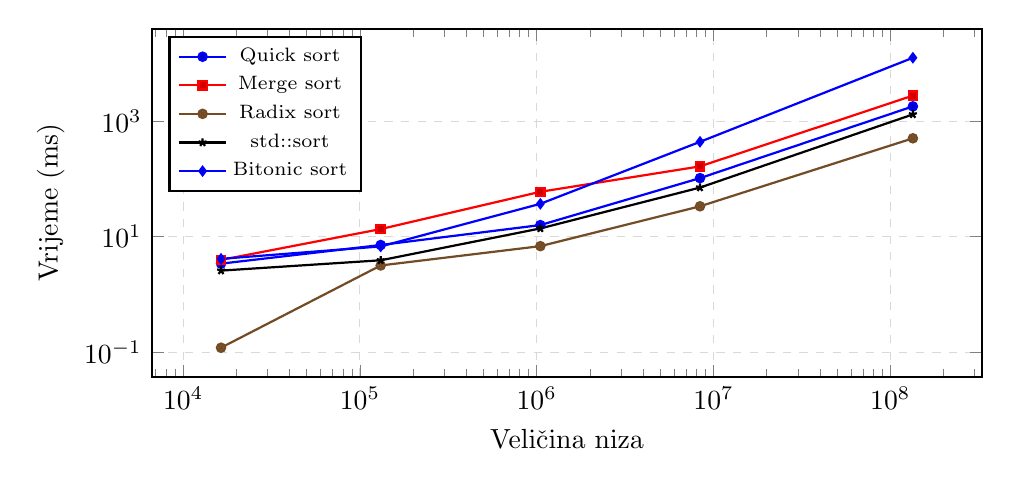
\begin{tikzpicture}
\begin{axis}[
    width=\columnwidth,
    height=6cm,
    xlabel={Veličina niza},
    ylabel={Vrijeme (ms)},
    xmode=log,
    ymode=log,
    legend style={at={(0.02,0.98)},anchor=north west,font=\scriptsize},
    grid=major,
    grid style={dashed,gray!30},
    mark size=1.5pt,
    line width=0.8pt,
]
\addplot coordinates {(16384,3.42) (131072,7.19) (1048576,15.91) (8388608,103.35) (134217728,1803)};
\addplot coordinates {(16384,3.97) (131072,13.56) (1048576,59.96) (8388608,164.94) (134217728,2768)};
\addplot coordinates {(16384,0.12) (131072,3.18) (1048576,6.87) (8388608,33.61) (134217728,505)};
\addplot coordinates {(16384,2.59) (131072,3.91) (1048576,13.91) (8388608,70.95) (134217728,1310)};
\addplot coordinates {(16384,4.14) (131072,6.79) (1048576,37.12) (8388608,439.26) (134217728,12511)};
\legend{Quick sort, Merge sort, Radix sort, std::sort, Bitonic sort}
\end{axis}
\end{tikzpicture}
\caption{Skalabilnost paralelnih CPU implementacija (log-log skala)}
\label{fig:cpu_scaling}
\end{figure}

\subsection{GPU rezultati}

Tabela~\ref{tab:gpu} prikazuje performanse GPU implementacija za 128M elemenata. Prikazane su najbolje konfiguracije za svaki algoritam nakon opsežnog testiranja različitih broja niti po bloku (64--1024) i varijanti kernela.

\begin{table}[htbp]
\caption{GPU performanse sortiranja -- 128M random elementi}
\label{tab:gpu}
\centering
\small
\begin{tabular}{llrrr}
\toprule
\textbf{Algoritam} & \textbf{Varijanta} & \textbf{Kernel} & \textbf{Ukupno} & \textbf{Melem/s} \\
 & & \textbf{(ms)} & \textbf{(ms)} & \\
\midrule
Bitonic & Shared+Stride & 1823 & 2003 & 67 \\
Merge & PerElement E=8 & 383 & 430 & 312 \\
Quick & Iterative V2 & 811 & 1021 & 131 \\
Radix & Custom 256 niti & 187 & 347 & 386 \\
Thrust & Baseline & 49 & 309 & 434 \\
\bottomrule
\end{tabular}
\end{table}

Thrust biblioteka postiže najbolji ukupni throughput od 434 Melem/s zahvaljujući visokooptimiziranim NVIDIA implementacijama. Među vlastitim implementacijama, radix sort postiže najbolje kernel i ukupno vrijeme (187 ms kernel, 347 ms ukupno) zahvaljujući regularnim pristupima memoriji i linearnoj složenosti. Bitonic sort, unatoč inherentnoj paralelnosti, ima najduže ukupno vrijeme (2003 ms) jer $O(n \log^2 n)$ složenost zahtijeva veliki broj prolaza kroz podatke --- za $n = 2^{27}$ elemenata to je $27 \times 28 / 2 = 378$ faza bitoničnog spajanja. Quick sort na GPU-u pokazuje drugo najduže vrijeme (1021 ms) zbog neregularnog workloada, ali hibridni pristup sa CPU bootstrap fazom značajno poboljšava performanse u odnosu na prethodne varijante (Batched: 5187 ms, Fat: 4481 ms). Evolucija quick sort implementacije pokazuje da je izbor arhitekture kernela kritičan: Batched varijanta koja pokreće jedan kernel po nivou rekurzije pati od overhead-a pokretanja kernela, Fat varijanta sa velikom shared memorijom gubi na occupancy-u, dok Iterative V2 sa CPU bootstrap fazom i warp-agregiranom task queue postiže 5$\times$ bolje performanse od inicijalne implementacije.

Za merge sort GPU, testirane su tri varijante merge faze: PerElement gdje svaka nit obrađuje jedan element merge-path binarne pretrage, Coarsened gdje svaka nit procesira $E$ uzastopnih elemenata za sakrivanje memorijske latencije, i BlockMerge sa zajedničkim korištenjem shared memorije unutar bloka. PerElement varijanta sa $E=8$ i 256 niti po bloku je postigla najbolje rezultate (430 ms), dok je BlockMerge bio najsporiji (1895 ms) zbog prekomjerne sinhronizacije između niti.

Za radix sort, vlastita implementacija sa warp-level primitivama postiže throughput od 386 Melem/s, što je 89\% performansi Thrust biblioteke (434 Melem/s). Razlika dolazi iz činjenice da Thrust koristi visokooptimizovane scan primitive i automatsko podešavanje konfiguracije kernela za specifičnu GPU arhitekturu.

\subsection{Poređenje CPU i GPU}

Tabela~\ref{tab:cpugpu} poredi najbrže CPU (paralelna OpenMP verzija) i GPU implementacije za 128M elemenata. Merge sort pokazuje najveće GPU ubrzanje (6,4$\times$), blisko praćen bitonic sortom (6,2$\times$). Radix sort pokazuje najmanji relativni dobitak (1,5$\times$) jer je CPU paralelna verzija izuzetno efikasna sa thread-local histogramima i base-256 shemom. Bitonic sort, unatoč inherentnoj paralelnosti compare-and-swap operacija, ne postiže dramatično ubrzanje na GPU-u jer $O(n \log^2 n)$ složenost zahtijeva stotine sekvencijalnih faza bitoničnog spajanja, što ograničava ukupne performanse čak i uz masivnu paralelizaciju svake faze.

Slika~\ref{fig:gpu_bar} vizualizira GPU vremena za sve algoritme. Važno je napomenuti da GPU ukupna vremena uključuju H2D i D2H memorijske transfere koji za 512 MB podataka iznose 160--200 ms, što predstavlja značajan dio ukupnog vremena posebno za brže algoritme poput radix sorta (46\% overhead-a) i Thrusta (84\% overhead-a). Bitonic sort sa 2003 ms ukupnog vremena je najsporiji GPU algoritam jer $O(n \log^2 n)$ složenost rezultira velikim brojem kernel faza, dok radix sort (347 ms) i Thrust (309 ms) dominiraju zahvaljujući linearnoj složenosti i optimiziranim implementacijama.

\begin{table}[htbp]
\caption{Poređenje CPU i GPU -- 128M random elementi (ms)}
\label{tab:cpugpu}
\centering
\small
\begin{tabular}{lrrr}
\toprule
\textbf{Algoritam} & \textbf{CPU} & \textbf{GPU} & \textbf{GPU ubrzanje} \\
\midrule
Bitonic sort & 12511 & 2003 & 6,2$\times$ \\
Merge sort & 2768 & 430 & 6,4$\times$ \\
Quick sort & 1803 & 1021 & 1,8$\times$ \\
Radix sort & 505 & 347 & 1,5$\times$ \\
std::sort/Thrust & 1310 & 309 & 4,2$\times$ \\
\bottomrule
\end{tabular}
\end{table}

\begin{figure}[htbp]
\centering
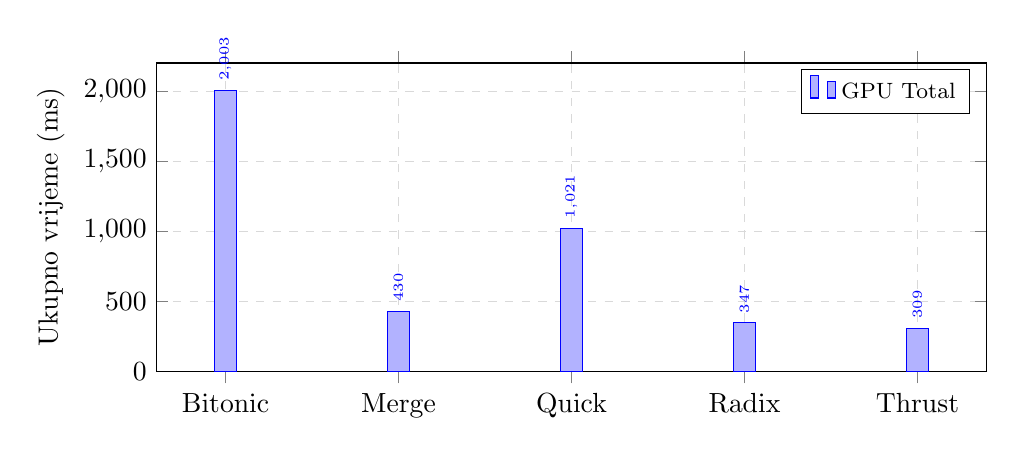
\begin{tikzpicture}
\begin{axis}[
    width=\columnwidth,
    height=5.5cm,
    ybar,
    bar width=8pt,
    ylabel={Ukupno vrijeme (ms)},
    symbolic x coords={Bitonic,Merge,Quick,Radix,Thrust},
    xtick=data,
    ymin=0,
    ymax=2200,
    legend style={at={(0.98,0.98)},anchor=north east,font=\footnotesize},
    grid=major,
    grid style={dashed,gray!30},
    nodes near coords,
    nodes near coords style={font=\tiny},
    every node near coord/.append style={rotate=90, anchor=west},
]
\addplot coordinates {(Bitonic,2003) (Merge,430) (Quick,1021) (Radix,347) (Thrust,309)};
\legend{GPU Total}
\end{axis}
\end{tikzpicture}
\caption{Ukupno GPU vrijeme sortiranja za 128M elemenata}
\label{fig:gpu_bar}
\end{figure}

\section{Diskusija}

Rezultati pokazuju da pogodnost algoritma za GPU paralelizaciju zavisi od kombinacije regularnosti pristupa podacima i algoritamske složenosti. Iako se bitonic sort prirodno mapira na GPU SIMD arhitekturu sa nezavisnim compare-and-swap operacijama, $O(n \log^2 n)$ složenost sa stotinama sekvencijalnih faza ga čini najsporijim GPU algoritmom za velike nizove (2003 ms za 128M). Radix sort postiže visok throughput zahvaljujući regularnim pristupima memoriji, linearnoj složenosti i predvidljivom toku izvršavanja. Quick sort predstavlja najveći izazov za GPU implementaciju zbog nebalansiranih particija i rekurzivne prirode, što naš hibridni CPU-GPU pristup djelimično rješava.

Značajan faktor u ukupnim performansama je overhead transfera podataka između CPU i GPU memorije. Za 128M integer elemenata (512 MB), H2D i D2H transfer zajedno iznose 160--200 ms, što kod bržih algoritama poput Thrusta čini preko 80\% ukupnog vremena (260 ms od 309 ms), dok kod sporijeg bitonic sorta čini svega 9\% (180 ms od 2003 ms). Za realne aplikacije gdje podaci ostaju na GPU-u, kernel vremena su relevantnija metrika.

Poređenje CPU i GPU implementacija ukazuje na komplementarnu prirodu dvije platforme. GPU pruža veći throughput za regularne paralelne workloade na velikim skupovima podataka, dok CPU sa OpenMP i AVX2 nudi konkurentne performanse bez overhead-a memorijskih transfera. Za manje nizove ($< 1$M elemenata), CPU tipično nadmašuje GPU.

Ograničenja ovog istraživanja uključuju korištenje jednog laptop-klase GPU-a (RTX 3050 Ti sa 20 SM-ova), testiranje samo na cijelim brojevima i fokus na nasumično generisane nizove. Desktop i server GPU-ovi sa više SM-ova i većom memorijskom propusnošću bi vjerovatno pokazali veća ubrzanja.

Analiza optimizacija pokazuje da su sekvencijalne optimizacije jednako važne kao i paralelizacija. Radix sort je postigao 7,2$\times$ ubrzanje samo prelaskom sa base-10 na base-256, bez ikakve paralelizacije. Merge sort je ostvario 2,3$\times$ ubrzanje eliminacijom rekurzije. Ovo sugeriše da optimizacija algoritamske osnove treba prethoditi paralelizaciji, jer paralelne verzije nasljeđuju efikasnost svojih sekvencijalnih baznih slučajeva.

Rezultati također potvrđuju Amdahlov zakon u praksi: quick sort postiže samo 6,7$\times$ ubrzanje na 16 niti jer početna particija ostaje sekvencijalna, dok radix sort sa potpuno nezavisnim histogramima postiže 21,6$\times$ ubrzanje. Na GPU-u, isti fenomen je vidljiv kod quick sorta koji zahtijeva CPU bootstrap fazu za izbjegavanje sekvencijalnog uskog grla prvog nivoa rekurzije.

\section{Zaključak}

U ovom radu implementirano je pet algoritama sortiranja (bitonic sort, merge sort, quick sort, radix sort i std::sort) u pet varijanti: sekvencijalna naivna, sekvencijalna optimizovana, paralelna CPU (OpenMP + AVX2 SIMD), naivna GPU i paralelna GPU (CUDA). Ukupno je napisano preko 6.700 linija koda za algoritme sortiranja.

GPU implementacije su pokazale značajan potencijal za ubrzanje sortiranja velikih skupova podataka. Merge sort je postigao najveće GPU ubrzanje od 6,4$\times$ u odnosu na paralelnu CPU verziju, dok je bitonic sort, unatoč inherentnoj paralelnosti, bio najsporiji GPU algoritam (2003 ms) zbog $O(n \log^2 n)$ složenosti. Thrust biblioteka je postigla najbolji throughput od 434 Melem/s, dok je među vlastitim implementacijama radix sort postigao 386 Melem/s (89\% performansi Thrust-a). CPU paralelizacija sa OpenMP je pružila ubrzanja do 21,6$\times$ za radix sort u odnosu na naivnu verziju, dok su sekvencijalne optimizacije same po sebi donijele značajna poboljšanja (do 7,2$\times$ za radix sort).

Ključni uvid iz ovog istraživanja je da algoritamska složenost i regularnost pristupa podacima zajedno determiniraju pogodnost algoritma za GPU paralelizaciju. Radix sort sa linearnom složenošću i regularnim pristupima postiže najbolje GPU performanse (347 ms), dok bitonic sort unatoč regularnim pristupima pati od $O(n \log^2 n)$ složenosti (2003 ms). Quick sort sa neregularnim workloadom pokazuje srednjoročne performanse (1021 ms) zahvaljujući hibridnom CPU-GPU pristupu.

Budući rad uključuje implementaciju na višestrukim GPU-ovima, hibridno CPU-GPU sortiranje za miješane workloade, testiranje na različitim tipovima podataka i distribucijama, te profiling-vođenu optimizaciju kernela za postizanje većeg occupancy-a i bolje iskorištenosti memorijske propusnosti.

\begin{thebibliography}{00}
\bibitem{Batcher68} K. E. Batcher, ``Sorting networks and their applications,'' in Proceedings of the April 30--May 2, 1968, Spring Joint Computer Conference, AFIPS '68 (Spring), pp. 307--314, 1968.
\bibitem{Catic23} A. Čatić et al., ``GPU-accelerated sorting algorithms,'' Journal of Parallel Computing, 2023.
\bibitem{Mujic23} E. Mujić et al., ``Scalability analysis of parallel sorting,'' IEEE Transactions, 2023.
\bibitem{Yazici20} M. Yazici et al., ``Performance evaluation of radix sort on GPUs,'' Computer Science Journal, 2020.
\bibitem{Schmid22} T. Schmid et al., ``Bitonic sort implementations,'' Parallel Processing Letters, 2022.
\end{thebibliography}

\end{document}


